\chapter{Introduction}

\label{introduction}


%what is open science?
Open Science 

Open Science is the practice of science in such a way that others can collaborate and contribute, where research data, lab notes and other research processes are freely available, under terms that enable reuse, redistribution and reproduction of the research and its underlying data and methods.

The movement to make scientific research, data and dissemination accessible to all levels of an inquiring society

\begin{figure*}[ht]
  \centering
  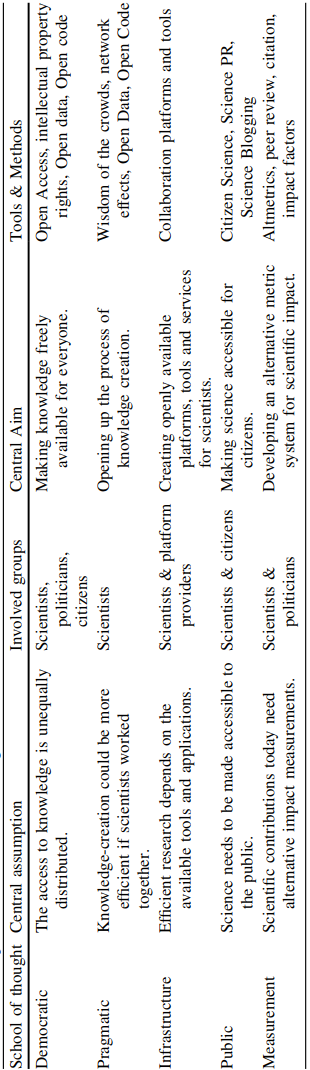
\includegraphics[width=\textwidth,height=\textheight,keepaspectratio]{figures/schools.png}%Methodology_May17th.png}
  \caption{Five Open Science schools of thought}
  \label{tab:method}
  \end{figure*} 

%why open science is important?
Open Science is increasingly important in current science world and has emerged as a framework to improve the quality of scientific analysis.

"Mostly due to current methods capture and data 
malpractice, approximately 
50\% of all research data 
and experiments is considered 
not reproducible, 
and the vast majority (likely over 80\%) of data 
never makes it to a trusted and sustainable 
repository.”~\cite{ayris2016realising} 



% how open science is defined? any other definition that FAIR?
As an open science study, the resources and the analysis should guarantee the FAIR~\cite{wilkinson2016fair} principles to be Findable, Accessible, Interoperable, and Reusable for the scientists and the researchers. 

%open science in nouroscuience meaning
In neuroscience studies the resources are including datasets, neuroimaging pipelines and tools, and analysis applied on the data.

%data sharing in neuroscience

% tools are required to process the data, tool sharing in neuroscience (harfaye tristan)


% related platforms for data and tool sharing in neuroscience
As a result, many platforms have emerged such as OpenNeuro, NeuroImaging Tools \& Resources Collaboratory (NITRC) and Canadian Open Neuroscience Platform (CONP) to facilitate data and tool sharing.


%the problem we focused on?
Although there are many platforms for data and tool sharing in neuroscience, there is still lacking of a system to help users  bridging the datasets and tools together which is the goal of this thesis. To help the users with such system we will adopt an approach based on recommender systems since there have been many successful works on recommender systems in past 15 years such as Netflix~\cite{bennett2007netflix} and Amazon~\cite{7927889}. There are two main strategies for recommender systems, Collaborative Filtering~\cite{rajaraman2011mining} and Content-based Filtering~\cite{pazzani2007content}. We selected collaborative filtering to implement a system to recommend datasets to pipelines and pipelines to datasets in the field of neuroimaging. Consistently with our motivating use case, we focused on the available neuroscience pipelines and datasets in CONP. 

% what will be in this thesis?

This thesis is organized as follows, in chapter two we explain the details about the required components and background knowledge, chapter three represents our approach, and in chapter four we expand the conclusion. 


